\section{EDA}

Para el análisis del DataFrame creado en la parte anterior, primero se categorizan las variables obtenidas en numéricas, categóricas y las numéricas con el UPZ agregado. Para las variables categóricas, vale la pena mencionar la relación de precio por metro cuadrado con la variable \comillas{furnished}, para la cual se realizó el siguiente violin plot:

\begin{multicols}{2}
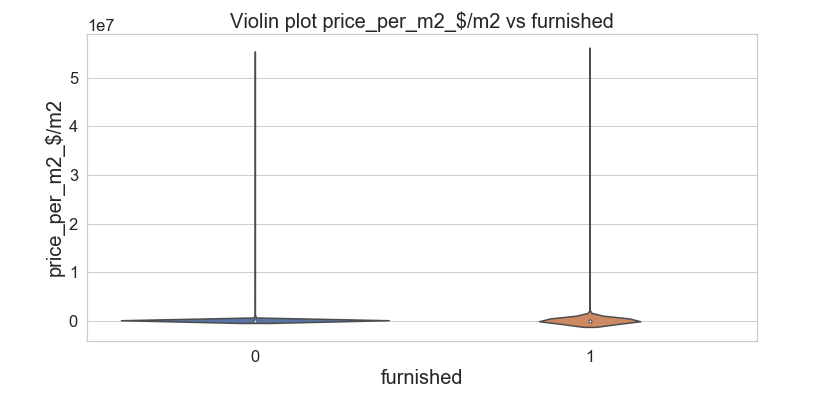
\includegraphics[scale = 0.4]{img/ejemplos/P2-2-1.png}

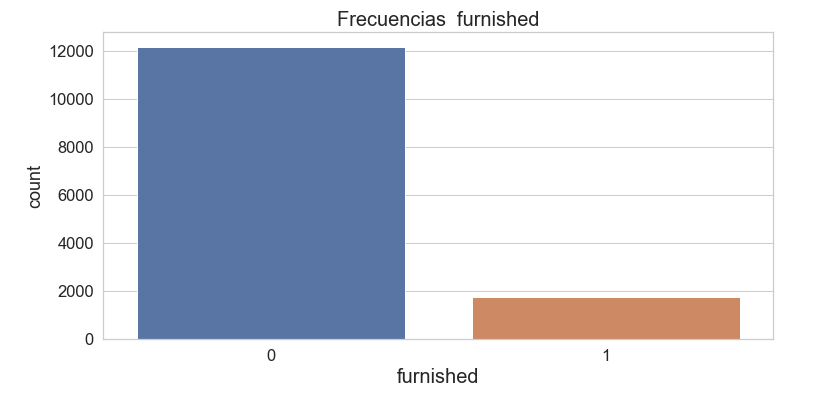
\includegraphics[scale = 0.4]{img/ejemplos/P2-2-2.png}
\end{multicols}

El segundo gráfico muestra la frecuencia de \comillas{furnished} en base a la notación puesta en la parte 1. Se puede apreciar que hay muchos datos que no provienen de \comillas{furnished}, pero la distribución de ambas según el precio por metro cuadrado se concentra de forma similar.

Otro caso interesante es el de la relación de el precio por metro cuadrado y el número de habitaciones

 \begin{center}
     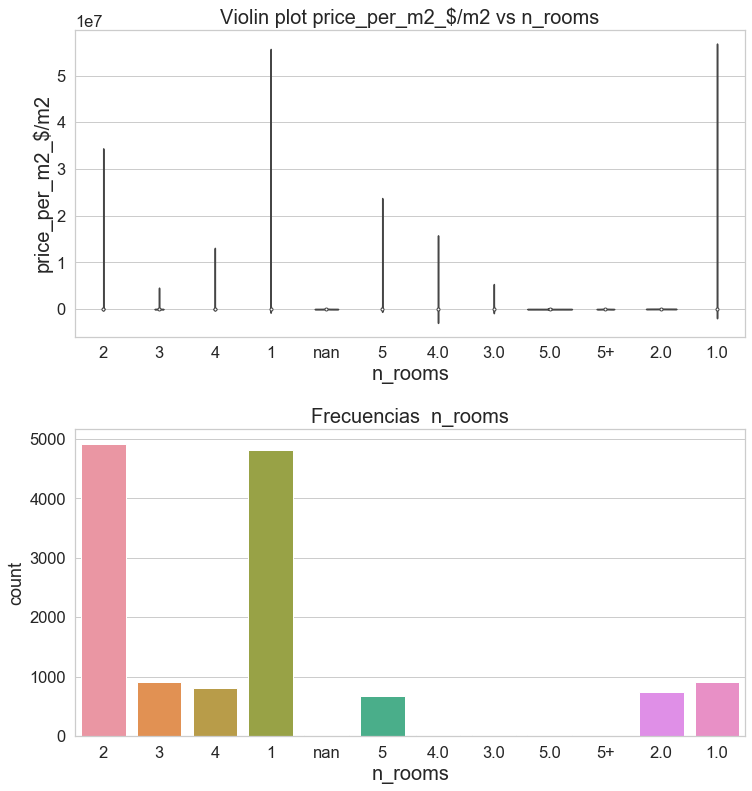
\includegraphics[scale = 0.3]{img/ejemplos/P2-2-3.png}
 \end{center}
 se puede observar que la mayor cantidad de habitaciones es de 1 y 2, y son las que alcanzan tienen mayores precios por metro cuadrado.

Para recategorizar la variable código de UPZ se utilizará kmeans en el promedio de cada selección de código UPZ, para luego dar las etiquetas entregadas por esta función.

\begin{center}
    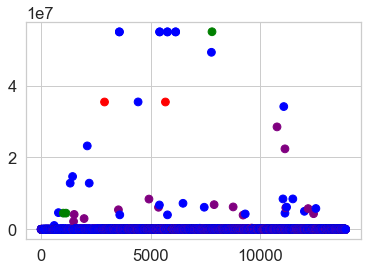
\includegraphics[scale = 0.5]{img/ejemplos/kluster.png}
\end{center}

En el gráfico anterior, si bien no se ven tan explicito, a diferencia de otros cluster que se probaron, estos tienen el mismo código UPZ. En otras palabras es una selección más gruesa que contiene los códigos.